\section{Representations of \texorpdfstring{$\sl_2$}{sl(2)}}

From now on, all algebras and representations are over $\C$ (an algebraically
closed field of characteristic $0$). Periodically we'll mention which results
don't need this.

Recall the basis of $\sl_2$ was
$e = \bigl(\begin{smallmatrix} 0 & 1 \\ 0 & 0 \end{smallmatrix}\bigr)$,
$h = \bigl(\begin{smallmatrix} 1 & 0 \\ 0 & -1 \end{smallmatrix}\bigr)$, and
$f = \bigl(\begin{smallmatrix} 0 & 0 \\ 1 & 0 \end{smallmatrix}\bigr)$, with
commutation relations $[e, f] = h$, $[h, e] = 2e$, $[h, f] = -2f$.

For the next while, we will be proving the following.

\begin{theorem}\leavevmode
\begin{enumerate}
  \item For all $n \geq 0$ there exists a unique irreducible representation of
    $\g = \sl_2$ of dimension $n + 1$. (Recall $L(n)$ from the previous
    lecture; these are the only ones.)
  \item Every finite-dimensional representation of $\sl_2$ is a direct sum of
    irreducible representations.
\end{enumerate}
\end{theorem}

Let $V$ be a representation of $\sl_2$.

\begin{definition}
The \emph{$\lambda$-weight space} for $V$ is
$V_\lambda = \setc{v \in V}{hv = \lambda v}$, the eigenspace of $h$ with
eigenvalue $\lambda$.
\end{definition}

\begin{example}
In $L(n)$, we had $L(n)_\lambda = \C x^iy^j$ for $\lambda = i - j$.
\end{example}

Let $v \in V_\lambda$, and consider $ev$. We have
\[
  hev = (he - eh + eh)v = [h, e]v + e(hv) = 2ev + e\lambda v = (\lambda + 2)ev.
\]
That is, if $v \in V_\lambda$ then $ev \in V_{\lambda+2}$, and similarly
$fv \in V_{\lambda-2}$. (These are clearly iff.)

We will think of this pictorially as a chain
\[
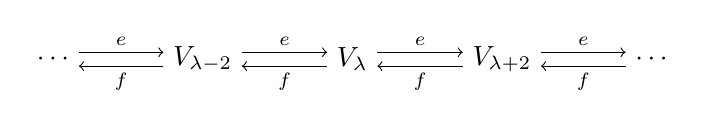
\begin{tikzpicture}[baseline=-3pt,x=1.9cm]
  \node (a) at (0,0) {$\cdots$};
  \node (b) at (1,0) {$V_{\lambda-2}$};
  \node (c) at (2,0) {$V_\lambda$};
  \node (d) at (3,0) {$V_{\lambda+2}$};
  \node (z) at (4,0) {$\cdots$};
  \foreach \x/\y in {a/b,b/c,c/d,d/z} {
    \draw[->] ([yshift=2.5pt]\x.east) -- node[above=-1pt]{\scriptsize $e$} ([yshift=2.5pt]\y.west);
    \draw[<-] ([yshift=-2.5pt]\x.east) -- node[below=-1pt]{\scriptsize $f$} ([yshift=-2.5pt]\y.west);
  }
\end{tikzpicture}
\]
E.g., in $L(n)$ we had $x^iy^j$ sitting in the place of the $V_\lambda$'s, and
the chain went from $\lambda = n$ to $\lambda = -n$:
\[
\begin{array}{*{13}{c}}
  V_n & \longleftrightarrow & V_{n-2} & \longleftrightarrow & V_{n-4} &
  \longleftrightarrow & \cdots & \longleftrightarrow & V_{-(n-4)} &
  \longleftrightarrow & V_{-(n-2)} & \longleftrightarrow & V_{-n}\\[2pt]
  \langle x^n\rangle & \rightleftarrows & \langle x^{n-1}y\rangle &
  \rightleftarrows & \langle x^{n-2}y^2\rangle & \rightleftarrows & \cdots &
  \rightleftarrows & \langle x^2y^{n-2}\rangle & \rightleftarrows &
  \langle xy^{n-1}\rangle & \rightleftarrows & \langle y^n\rangle
\end{array}
\]
(Note that the string for $L(n)$ has $n + 1$ elements.)

\begin{definition}
If $v \in V_\lambda \cap \ker e$, i.e.\ $hv = \lambda v$ and $ev = 0$, then we
say that $v$ is a \emph{highest-weight vector} of weight $\lambda$.
\end{definition}

\begin{lemma}
Let $V$ be a representation of $\sl_2$ and $v \in V$ a highest-weight vector
of weight $\lambda$. Then $W = \langle v, fv, f^2v, \dots\rangle$ is an
$\sl_2$-invariant subspace, i.e.\ a subrepresentation.
\end{lemma}

\begin{proof}
We need to show $hW \subseteq W$, $fW \subseteq W$, and $eW \subseteq W$.
Note that $fW \subseteq W$ by construction. Further, since $v \in V_\lambda$,
we saw above that $f^kv \in V_{\lambda - 2k}$, and so $hW \subseteq W$ as well.
Finally,
\begin{align*}
  ev &= 0 && \in W\\
  efv &= ([e, f] + fe)v = hv + f(0) = \lambda v && \in W\\
  ef^2v &= ([e, f] + fe)fv = (\lambda - 2)fv + f(\lambda v) = (2\lambda - 2)fv && \in W\\
  ef^3v &= ([e, f] + fe)f^2v = (\lambda - 4)f^2v + f(2\lambda - 2)fv = (3\lambda - 6)f^2v && \in W
\end{align*}
and so on.
\end{proof}

\begin{exercise}
$ef^nv = n(\lambda - n + 1)f^{n-1}v$ for $v$ a highest-weight vector of weight
$\lambda$.
\end{exercise}

\begin{lemma}
Let $V$ be a finite-dimensional representation of $\sl_2$ and $v \in V$ a
highest-weight vector of weight $\lambda$. Then $\lambda \in \Z_{\geq 0}$.
\end{lemma}

\begin{remark}
Somehow, the integrality condition is the Lie algebra remembering something
about the topology of the group. (Saying what this ``something'' is more
precisely is difficult.)
\end{remark}

\begin{proof}
Note that the $f^kv$ all lie in different eigenspaces of $h$, so if they are
all nonzero then they are linearly independent. Since $\dim V < \infty$, we
conclude that there exists a $k$ such that $f^kv \neq 0$ and $f^{k+r}v = 0$ for
all $r \geq 1$. Then by the above exercise,
\[
  0 = ef^{k+1}v = (k + 1)(\lambda - k)f^kv,
\]
from which $\lambda = k$, a nonnegative integer.
\end{proof}

\begin{proposition}
If $V$ is a nonzero finite-dimensional representation of $\sl_2$, it has a
highest-weight vector.
\end{proposition}

\begin{proof}
We're over $\C$, so we can pick some eigenvector $v$ of $h$, of eigenvalue
$\lambda$ say. Now apply $e$ to it repeatedly: $v, ev, e^2v, \dots$ belong to
different eigenspaces of $h$, so if they are nonzero, they are linearly
independent. Therefore, there must be some $k$ such that $e^kv \neq 0$ but
$e^{k+r}v = 0$ for all $r \geq 1$. Then $e^kv$ is a highest-weight vector of
weight $\lambda + 2k$.
\end{proof}

\begin{corollary}
If $V$ is an irreducible representation of $\sl_2$ then $\dim V = n + 1$ for
some $n \geq 0$, and $V$ has a basis $v_0, v_1, \dots, v_n$ on which $\sl_2$
acts as $hv_i = (n - 2i)v_i$; $fv_i = v_{i+1}$ (with $fv_n = 0$); and
$ev_i = i(n - i + 1)v_{i-1}$. In particular, there exists a unique
$(n+1)$-dimensional irreducible representation, which must be isomorphic to
$L(n)$.
\end{corollary}

\begin{exercise}
Work out how this basis is related to the basis we previously had for $L(n)$.
\end{exercise}

\lecture{4} We will now show that every finite-dimensional representation of
$\sl_2(\C)$ is a direct sum of irreducible representations, or
(equivalently) the category of finite-dimensional representations of
$\sl_2(\C)$ is \emph{semisimple}, or (equivalently) every representation of
$\sl_2(\C)$ is \emph{completely reducible}.

Morally, we've shown that every such representation consists of ``strings''
descending from the highest weight, and we'll now show that these strings
don't interact. We'll first show that they don't interact when they have
different highest weights (easier) and then that they also don't interact when
they have the same highest weight (harder).

We will also show that $h$ acts diagonalisably on every finite-dimensional
representation, while $e$ and $f$ are nilpotent. In fact,

\begin{remark}
\[
  \C h = \Bigl\{ \begin{pmatrix} a & \\ & -a \end{pmatrix} \Bigr\}
       = \Lie \Bigl\{ \begin{pmatrix} t & \\ & t^{-1} \end{pmatrix} \Bigr\}
       \subset \Lie(SL_2),
\]
where $\bigl\{\bigl(\begin{smallmatrix} t & \\ & t^{-1}\end{smallmatrix}\bigr)\bigr\}$
is the maximal torus inside $SL_2$. As for $\C^\times$, the representations
here should correspond to integers. In some hazy way, the fact that we are
picking out the representations of a circle and not any other $1$-dimensional
Lie group is a sign of the Lie algebra remembering something about the group.
(Saying what it is remembering and how is a hard question.)
\end{remark}

\begin{example}
Recall that $\C[x, y]$ is a representation of $\sl_2$ via the action by
differential operators, and is a direct sum of the representations $L(n)$.
\end{example}

\begin{exercise}
Show that the formulae $e = x\frac{\partial}{\partial y}$,
$f = y\frac{\partial}{\partial x}$,
$h = x\frac{\partial}{\partial x} - y\frac{\partial}{\partial y}$ give a
representation of $\sl_2$ on $x^\lambda y^\mu\C[x/y, y/x]$ for any
$\lambda, \mu \in \C$, and describe the submodule structure.
\end{exercise}

\begin{definition}
Let $V$ be a finite-dimensional representation of $\sl_2$. Define
$\Omega = ef + fe + \frac12 h^2 \in \End(V)$ to be the \emph{Casimir} of
$\sl_2$.
\end{definition}

\begin{lemma}
$\Omega$ is central; that is, $e\Omega = \Omega e$, $f\Omega = \Omega f$, and
$h\Omega = \Omega h$.
\end{lemma}

\begin{exercise}
Prove it. For example,
\begin{align*}
  e\Omega = e\Bigl(ef + fe + \frac12 h^2\Bigr)
    &= e(ef - fe) + 2(efe) + \frac12(eh - he)h + \frac12 heh\\
    &= 2efe + \frac12 heh\\
    &= (fe - ef)e + 2efe + \frac12 h(he - eh) + \frac12 heh = \Omega e.
\end{align*}
\end{exercise}

Observe that we can write
$\Omega = (ef - fe) + 2fe + \frac12 h^2 = (\frac12 h^2 + h) + 2fe$. This will
be useful later.

\begin{corollary}
If $V$ is an irreducible representation of $\sl_2$, then $\Omega$ acts on $V$
by a scalar.
\end{corollary}

\begin{proof}
Schur's lemma.
\end{proof}

\begin{lemma}
Let $L(n)$ be the irreducible representation of $\sl_2$ with highest weight
$n$. Then $\Omega$ acts on $L(n)$ by $\frac12 n^2 + n$.
\end{lemma}

\begin{proof}
It suffices to check this on the highest-weight vector $v$ (so $hv = nv$ and
$ev = 0$). Then
\[
  \Omega v = \Bigl(\frac12 h^2 + h + 2fe\Bigr)v = \Bigl(\frac12 n^2 + n\Bigr)v.
\]
Since $\Omega$ commutes with $f$ and $L(n)$ is spanned by the $f^iv$, we could
conclude directly (without using Schur's lemma) that $\Omega$ acts by this
scalar.
\end{proof}

Observe that if $L(n)$ and $L(m)$ are irreducible representations with
different highest weights, then $\Omega$ acts by different scalars on them
(since $\frac12 n(n + 2)$ is increasing in $n \geq 0$).

\begin{definition}
Let $V$ be a finite-dimensional representation of $\sl_2$. Set
\[
  V^\lambda = \setc{v \in V}{(\Omega - \lambda)^{\dim V}v = 0}.
\]
This is the \emph{generalised eigenspace of $\Omega$ with eigenvalue
$\lambda$}.
\end{definition}

\begin{claim}
Each $V^\lambda$ is a subrepresentation for $\sl_2$.
\end{claim}

\begin{proof}
Let $x \in \sl_2$ and $v \in V^\lambda$. Because $\Omega$ is central, we have
\[
  (\Omega - \lambda)^{\dim V}(xv) = x(\Omega - \lambda)^{\dim V}v = 0,
\]
so $xv \in V^\lambda$ as well.
\end{proof}

Now, if $V^\lambda \neq 0$, then $\lambda = \frac12 n^2 + n$, and $V^\lambda$
is somehow ``glued together'' from copies of $L(n)$. More precisely:

\begin{definition}
Let $W$ be a finite-dimensional $\g$-module. A \emph{composition series} for
$W$ is a sequence of submodules
\[
  0 = W_0 \subseteq W_1 \subseteq \dots \subseteq W_r = W
\]
such that each $W_i/W_{i-1}$ is an irreducible module.
\end{definition}

\begin{example}\leavevmode
\begin{enumerate}
  \item $\g = \C$, $W = \C^r$, where $1 \in \C$ acts as
    \[
      \begin{pmatrix}
        0 & 1 &        &        &   \\
          & 0 & 1      &        &   \\
          &   & \ddots & \ddots &   \\
          &   &        & \ddots & 1 \\
          &   &        &        & 0
      \end{pmatrix}.
    \]
    Then there exists a unique composition series for $W$, namely
    \[
      0 \subset \langle e_1\rangle \subset \langle e_1, e_2\rangle \subset \dots
        \subset \langle e_1, e_2, \dots, e_r\rangle.
    \]
  \item On the other hand, if $\g = \C$ and $W = \C^r$ with the zero action
    (i.e.\ $1 \in \C$ acts by $0$), then any chain
    $0 \subset W_1 \subset \dots \subset W_r$ with $\dim W_i = i$ will be a
    composition series.
\end{enumerate}
\end{example}

\begin{lemma}
Composition series always exist.
\end{lemma}

\begin{proof}
We induct on the dimension of $W$. Take a nonzero irreducible submodule
$W_1 \subseteq W$; then $W/W_1$ has smaller dimension, so has a composition
series. Taking its preimage in $W$ and sticking $W_1$ in front will do the
trick.
\end{proof}

\begin{remark}
The factors $W_i/W_{i-1}$ are determined by $W$ up to isomorphism and
reordering (the Jordan--H\"older theorem).
\end{remark}

So, the precise statement is that $V^\lambda$ has a composition series with
quotients $L(n)$ for some fixed $n$. Indeed, take an irreducible submodule
$L(n) \subset V^\lambda$; note that $\Omega$ acts on $L(n)$ by
$\frac12 n^2 + n$, so we must have $\lambda = \frac12 n^2 + n$, or in other
words $n$ is uniquely determined by $\lambda$; and moreover, $\Omega$ acts on
$V^\lambda/L(n)$, and its only generalised eigenvalue there is still
$\lambda$, so we can repeat the argument.

\begin{claim}
$h$ acts on $V^\lambda$ with generalised eigenvalues in the set
$\{n, n - 2, \dots, -n\}$.
\end{claim}

\begin{proof}
This is a general fact about composition series. Let $h$ act on $W$ and let
$W' \subset W$ be invariant under this action, i.e.\ $hW' \subseteq W'$. Then
\begin{multline*}
  \{\text{generalised eigenvalues of } h \text{ on } W\}
  = \{\text{generalised eigenvalues of } h \text{ on } W'\}\\
  \cup \{\text{generalised eigenvalues of } h \text{ on } W/W'\}.
\end{multline*}
(You can see this by looking at the block upper triangular form of the matrix
of $h$.) Now since $V^\lambda$ is composed of copies of $L(n)$, the generalised
eigenvalues of $h$ must lie in that set.
\end{proof}

Note also that on the kernel of $e\colon V^\lambda \to V^\lambda$ the only
generalised eigenvalue of $h$ is $n$; that is, $(h - n)^{\dim V^\lambda}x = 0$
for $x \in V^\lambda \cap \ker e$. (This follows by applying the above
observation to the composition series intersected with $\ker e$.)

\lecture{5}

\begin{lemma}\leavevmode
\begin{enumerate}
  \item $hf^k = f^k(h - 2k)$.
  \item $ef^{n+1} = f^{n+1}e + (n + 1)f^n(h - n)$.
\end{enumerate}
\end{lemma}

\begin{proof}
We saw (1) already, and (2) is the next exercise.
\end{proof}

\begin{exercise}
Prove (2) (by induction; e.g.\ for $n = 0$ the claim is $ef = fe + h$).
\end{exercise}

\begin{proposition}
$h$ acts diagonalisably on $\ker e\colon V^\lambda \to V^\lambda$; in fact, it
acts as multiplication by $n$. That is,
\[
  \ker\bigl(e\colon V^\lambda \to V^\lambda\bigr) = (V^\lambda)_n
    = \setc{x \in V^\lambda}{hx = nx}.
\]
\end{proposition}

Recall we know that $\ker e$ is (in) the \emph{generalised} eigenspace of $h$
with eigenvalue $n$ (and after the first line of the proof, we will have
equality rather than just containment). We are showing that we can drop the
word ``generalised''.

\begin{proof}
If $hx = nx$ then $ex \in (V^\lambda)_{n+2} = 0$ (as the generalised
eigenvalues of $h$ on $V^\lambda$ are $n, n - 2, \dots, -n$), so
$x \in \ker e$.

Conversely, let $x \in \ker e$; we know $(h - n)^{\dim V^\lambda}x = 0$. By
the lemma above,
\[
  (h - n + 2k)^{\dim V^\lambda}f^kx = f^k(h - n)^{\dim V^\lambda}x = 0.
\]
That is, $f^kx$ belongs to the generalised eigenspace of $h$ with eigenvalue
$n - 2k$.

On the other hand, for any $y \in \ker e$, $y \neq 0 \implies f^ny \neq 0$.

\begin{remark}
This should be an obvious property of upper-triangular matrices, but we'll
work it out in full detail.
\end{remark}

Take $0 = W_0 \subset W_1 \subset \dots \subset W_r = V^\lambda$, the
composition series for $V^\lambda$ with quotients $L(n)$. There is an $i$ such
that $y \in W_i$, $y \notin W_{i-1}$. Let
$\overline{y} = y + W_{i-1} \in W_i/W_{i-1} \cong L(n)$. Then $\overline{y}$ is
a highest-weight vector in $L(n)$, and so $f^n\overline{y} \neq 0$ in $L(n)$.
Therefore, $f^ny \neq 0$.

Now, $f^{n+1}x$ belongs to the generalised eigenspace of $h$ with eigenvalue
$-n - 2$, so is equal to $0$ (as the generalised eigenvalues of $h$ on
$V^\lambda$ are $n, n - 2, \dots, -n$). Therefore,
\[
  0 = ef^{n+1}x = (n + 1)f^n(h - n)x + f^{n+1}ex = (n + 1)f^n(h - n)x.
\]
Now, $(h - n)x \in \ker e$ (it's still in the generalised eigenspace of $h$
with eigenvalue $n$, and $e(h - n)x = (h - n - 2)ex = 0$), so if
$(h - n)x \neq 0$ then $f^n(h - n)x \neq 0$, and then
$(n + 1)f^n(h - n)x \neq 0$ in characteristic $0$, a contradiction. Therefore,
$hx = nx$.
\end{proof}

We can now finish the proof of complete reducibility. Indeed, choose a basis
$w_1, w_2, \dots, w_k$ of $\ker e\colon V^\lambda \to V^\lambda$, and consider
the ``string'' generated by each $w_i$; that is, consider
\[
  \langle w_i, fw_i, f^2w_i, \dots, f^nw_i\rangle.
\]

\begin{exercise}
Convince yourself that these strings constitute a direct sum decomposition of
$V^\lambda$; that is, these are subrepresentations, nonintersecting, linearly
independent, and span everything.
\end{exercise}

Therefore, $h$ acts semisimply and diagonalisably on $V^\lambda$, and
therefore on all of $V$.

\begin{exercise}
Show that this is false in characteristic $p$. That is, show that the
irreducible representations of $\sl_2(\Fpbar)$ are no longer parametrised by
$n \in \N$ (none of them has dimension greater than $p$), and find a
representation of $\sl_2(\Fpbar)$ that does not decompose into a direct sum of
irreducibles.
\end{exercise}
